\chapter{Game AI}
%Babbage, Charles -- . . .every game of skill is susceptible of being played by an automaton.
%Minsky, Marvin -- It is not that the games and mathematical problems are chosen because they are clear and simple; rather it is that they give us, for the smallest initial structures, the greatest complexity, so that one can engage some really formidable situations after a relatively minimal diversion into programming. From Semantic Information Processing, p. 12. Cambridge, MA: MIT Press (1968).
% If you'd like to know, I can tell you that in your universe you move freely in three dimensions that you call space. You move in a straight line in a fourth, which you call time, and stay rooted to one place in a fifth, which is the first fundamental of probability. After that it gets a bit complicated, and there's all sort of stuff going on in dimensions thirteen to twenty-two that you really wouldn't want to know about. All you really need to know for the moment is that the universe is a lot more complicated than you might think, even if you start from a position of thinking it's pretty damn complicated in the first place. I can easily not say words like "damn" if it offends you. H2G2

%%% Some characteristics of Game AI
%%% high-level perception, commonsense reasoning, NLP, speech processing,
%%% gesture processing, planning \& counterplanning, cognitive modeling,
%%% plan recognition, soft real-time response, reactive behavior, teamwork,
%%% scheduling, path planning, spatial reasoning, temporal reasoning,
%%% opponent modeling, learning, knowledge acquisition

\begin{verse}\textit{
\\
David: What is the primary goal?\\
Joshua: You should know, Professor. You programmed me.\\
David: Oh, come on. What is the primary goal?\\
Joshua: To win the game.\\
} Wargames (1983)\end{verse}
%\lettrine[image=true, lines=3, findent=3pt, nindent=0pt]{lettrines/O.png}{r}
\lettrine{I}{s} the primary goal of game AI to win the game? ``Game AI'' is simultaneously a research topic and an industry standard practice, for which the main metric is the fun the players are having. Its uses range from character animation, to behavior modeling, strategic play, and a true gameplay component. In this chapter, we will give our educated guess about the goals of game AI, and review what exists for a broad category of games: abstract strategy games, partial information and/or stochastic games, different genres of computer games. Let us then focus on gameplay (from a player point of view) characteristics of theses games so that we can enumerate game AI needs. %%% XXX
%\lettrine[image=true, lines=3, findent=3pt, nindent=0pt]{lettrines/W.png}{hat} is game AI? What are the goals of AI in games? What are its characteristics? Why is game AI an interesting subject for research? 

%%%%%%%%%%%%%%%%%%%%%%%%%%%%%%%%%%%%%%%%%%%%%%%%%%%%%%%%%%%%%%%%%% 

\section{Goals of Game AI}
%\lettrine[lines=1, lhang=.3]{W}{hat} are the goals of game AI?
\subsection{NPC}
%\newacronym{npc}{NPC}{non-playing characters}
\newglossaryentry{npc}{name=NPC,description={non-playing characters: game AI controlled third party characters, which were not conceived to be played by humans by opposition to ``bots''}}\Gls{npc}*, also called ``mobs'', represent a massive volume of game AI, as even a lot of multi-player games have \gls{npc}. They really represents players that are not conceived to be played by humans, by opposition to ``bots'', which corresponds to human-playable characters controlled by an AI. \gls{npc} are an important part of ever more immersive single player adventures (The Elder Scrolls V: Skyrim), of cooperative gameplay (World of Warcraft, Left 4 Dead), or as helpers or trainers (``pets'', strategy games). \gls{npc} can be a core part of the gameplay as in Creatures or Black and White or dull ``quest giving poles'' as in a lot of role-playing games. They are of interest for the game industry, but also for robotics, to study human cognition and for artificial intelligence in the large. So, the first goal of game AI is perhaps just to make the artificial world seem alive: a paint is not much fun to play in.

\subsection{Win}
%%%Not solved: humans are the best
During the last decade, the video games industry has seen the emergence of ``e-sport''. It is the professionalization of specific competitive games at the higher levels, as in sports: with spectators, leagues, sponsors, fans and broadcasts. A %non-exhaustive 
list of major electronic sports games includes (but is not limited to): StarCraft: Brood War, Counter-Strike, Quake III, Warcraft III, Halo, StarCraft II. The first game to have had \newglossaryentry{pro-gamer}{name=pro-gamer,description={professional gamer, full-time job},plural=pro-gamers}\gloss{pro-gamer} was \newglossaryentry{Broodwar}{name=StarCraft: Brood War,description={a science fiction real-time strategy (RTS) game released in 1998 by Blizzard Entertainment}}\glos{Broodwar}, in Korea, with top players earning more than Korean top soccer players. Top players earn more than \$400,000 a year but the professional average is below, around \$50-60,000 a year \citep{TeamLiquidPGMIncome}, against the average South Korean salary at \$16,300 in 2010. Currently, Brood War is being slowly phased out to StarCraft II (still 4.9 millions players in South Korea in 2011 \citep{CitationNeeded}). There are TV channels broadcasting Brood War (OnGameNet, previously also MBC Game) or StarCraft II (GOM TV, streaming) and for which it constitutes a major chunk of the air time. %in 2010 in South Korea, the average salary for a professional StarCraft player was \$60,000 against the average salary at \$16,300\citep{StarCraftPGM}). 
``E-sport'' is important to the subject of game AI because it ensures competitiveness of the human players. It is less challenging to write a competitive AI for game played by few and without competitions than to write an AI for Chess, Go or StarCraft. E-sport, through the distribution of \newglossaryentry{replay}{name=replay,description={the record of all players' actions during a game, allowing the game engine to recreate the game state deterministically},plural=replays}``\gloss{replay}'' also ensures a constant and heavy flow of human player data to mine and learn from. Finally, cognitive science researchers (like the Simon Fraser University Cognitive Science Lab) study the cognitive aspects (attention, learning) of high level RTS playing\citep{CitationNeeded}.

Good human players, through their ability to learn and adapt, and through high-level strategic reasoning, are still undefeated. Single players are often frustrated by the \gls{npc} behaviors in non-linear (not fully scripted) games. Nowadays, video games AI can be used as part of the gameplay as a challenge to the player. 
This is not the case in most of the games though, in decreasing order of resolution of the problem\footnote{Particularly considering games with possible free worlds and ``non-linear'' storytelling, current RPG and MMORPG are often limited \textit{because} of the untracted ``world interacting \gls{npc}'' AI problem.}: fast \newglossaryentry{FPS}{name=FPS,description={First Person Shooter: egocentric shooter game, strong sub-genres are fast FPS, also called ``Quake-likes'', e.g. Quake III; and team/tactical FPS, e.g. Counter-Strike, Team Fortress 2}}\glos{FPS} (first person shooters), team FPS, \newglossaryentry{RPG}{name=RPG,description={Role Playing Game, e.g. Dungeons \& Dragons based Baldur's Gate}}\glos{RPG} (role playing games), \newglossaryentry{MMORPG}{name=MMORPG,description={Massively Multi-player Online Role Playing Game, distinct of RPG by the scale of cooperation sometimes needed to achieve a common goal, e.g. Dark Age of Camelot, World of Warcraft}}\glos{MMORPG} (Massively Multi-player Online RPG), \newglossaryentry{RTS}{name=RTS,description={Real-Time Strategy games are (mainly) allocentric economic and military simulations from an operational tactical/strategist commander viewpoint, e.g. Command \& Conquer, Age of Empires, StarCraft, Total Annihilation}}\glos{RTS} (Real-Time Strategy). These games in which artificial intelligences do not beat top human players on equal footing requires increasingly more cheats to even be a challenge (not for long as they mostly do not adapt). AI cheats encompass (but are not limited to):
\begin{itemize}
\item RPG \gls{npc} often have at least 10 times more hit points (health points) than their human counterparts in equal numbers,
\item FPS bots can see through walls and use perfect aiming,
\item RTS bots see through the ``fog of war'' and have free additional resources.
\end{itemize}
How do we build game robotic players (``bots'', AI, \gls{npc}) which can provide some challenge, or be helpful without being frustrating, while staying fun?


\subsection{Fun}
%%%Not solved: humans are the most fun to play with
The main purpose of gaming is entertainment. Of course, there are game genres like serious gaming, or the ``\newglossaryentry{gamification}{name=gamification,description={the use of game mechanics and game design to enhance non-game contexts}}\glos{gamification}'' of learning, but the majority of people playing games are having fun. Cheating AI are not fun, and so the \newglossaryentry{replayability}{name=replayability,description={replay value, entertainment value of playing the game more than once}}\glos{replayability} of single player games is very low. The vast majority of games which are still played after the single player mode are multi-player games, because humans are the most fun to play with. So how do we get game AI to be fun to play with? The answer seems to be 3-fold:
\begin{itemize}
\item For competitive and \newglossaryentry{PvP}{name=PvP,description={Players versus Players}}\glos{PvP}
(players versus players) games: improve game AI so that it can play well \textit{on equal footing with humans},
\item for cooperative and \newglossaryentry{PvE}{name=PvE,description={Players vs Environment}}\glos{PvE}
(players vs environment) games: optimize the AI for fun, ``epic wins'': the empowerment of playing your best and just barely winning,
\item give the AI all the tools to adapt the game to the players: \newglossaryentry{AIdirector}{name=AI directors,description={system that overlooks the behavior of the players to manage the intensity, difficulty and fun},plural=AI directors}\gloss{AIdirector} (as in \newglossaryentry{left4dead}{name=Left 4 Dead,description={a teamplay (cooperative vs AI) survival horror FPS in which players have to fight and escape zombie hordes}}\glos{left4dead} and \newglossaryentry{darkspore}{name=Dark Spore,description={a fast-paced, sci-fi action-RPG, with PvP and cooperative (vs AI) modes}}\glos{darkspore}), procedural content generation (e.g. automatic personalized Mario \citep{Shaker10AIIDE}).
\end{itemize}
In all cases, a good AI should be able to learn for the players' actions, recognize their behavior to deal with it in the most entertaining way. Examples for a few mainstream games: World of Warcraft instances or StarCraft II missions could be less predictable (less scripted) and always ``just hard enough'', Battlefield 3 or Call of Duty opponents could have a longer life expectancy (5 seconds in some cases), Skyrim's follower \gls{npc} could avoid blocking the player in doors, or going in front when she casts fireballs.

\subsection{Programming}
How do game developers want to deal with game AI programming? We have to understand the needs of industry game AI programmers: 
\begin{itemize}
    \item computational efficiency: most games are real-time systems, 3D graphics are computationally intensive, as a result the AI CPU budget is low,
    \item game designers often want to remain in control of the behaviors, so game AI programmers have to provide authoring tools,
    \item AI code has to scale with the state spaces while being debuggable,
    \item AI behaviors have to scale with the possible game states (which are not all predictable due to the presence of the human player),
    \item re-use accross games (game independant logic, at least libraries).
\end{itemize}
As a first approach, programmers can ``hard code'' the behaviors and their switches. For some structuring of such states and transitions, they can and do use state machines \citep{FSM_AIGameProgWisdom2003}. This solution does not scale well (exponential increase in the number of transitions), nor do they generate autonomous behavior, and they can be cumbersome for the game designers to interact with. Hierarchical FSM \citep{CitationNeeded} is a partial answer to these problems: they scale better due to the sharing of transitions between macro-states and are more readable for game designers who can zoom-in on macro/englobing states. They still represent way too much programming work for complex behavior and are not more autonomous than classic FSM. Planning (using a search heuristic in the states space) efficiently gives autonomy to virtual characters. Planners like hierarchical task networks (HTN \citep{Erol_htnplanning}, Armed Assault, Killzone 2 \citep{ArmA1_HTN,Killzone2_HTN}) or STRIPS (\citep{FikesSTRIPS}, F.E.A.R \citep{orkinGDC_FEAR}) generate complex behaviors in the space of the combinations of specified states, and the logic can be re-used accross games. The drawbacks can be a large computational budget (for many agents and/or a complex world), the difficulty to specify reactive behavior, and less (or harder) control from the game designers. Behavior trees (Halo 2 \citep{Isla}, Spore) are a popular in-between HTN and HFSM technique providing scability through a tree-like hierarchy, control through tree editing and some autonomy through a search heuristic.
A transversal technique for ease of use is to program game AI with a script (LUA, Python) or domain specific language (\newglossaryentry{DSL}{name=DSL,description={Domain Specific Language}}\glos{DSL}). From a programming or design point of view, it will have the drawbacks of the models it is based on. If everything is allowed (low-level inputs and outputs directly in the DSL), everything is possible at the cost of cumbersome programming, debugging and few re-use.

Even with scalable\footnote{both computationally and in the number of lines of codes to write to produce a new behavior} architectures like behavior trees or the autonomy that planning provides, there are limitations (burdens on programmers/designers or CPU/GPU):
\begin{itemize}
    \item complex worlds require either very long description of the state (in propositional logic) or high expressivity (higher order logics) to specify well-defined behaviors,
    \item the search space of possible actions increases exponentially with the volume and complexity of interactions with the world, thus requiring ever more efficient pruning techniques,
    \item once human players are in the loop (is it not the purpose of a game?), uncertainty has to be taken into account. Previous approaches can be ``patched'' to deal with uncertainty, at what cost?
\end{itemize}
Our thesis is that we can learn complex behaviors from exploration or observations (of human players) without the need to be explicitely programmed. Furthermore, the game designers can stay in control by choosing which demonstration to learn from and tuning parameters by hand if wanted. \citet{LeHy04} showed it in the case of FPS AI (Unreal Tournament), with \textit{inverse programming} to learn reactive behaviors from human demonstration. We extend it to tactical and even strategic behaviors.

%%%%%%%%%%%%%%%%%%%%%%%%%%%%%%%%%%%%%%%%%%%%%%%%%%%%%%%%%%%%%%%%%% 

\section{Single Player Games}

Single player games are not the main focus of our thesis, but they present a few interesting AI characteristics. They encompass all kinds of human cognitive abilities, from reflexes to higher level thinking.

\subsection{Action games}
%%% Mario, racing, PacMan
Platform games (Mario, Sonic), time attack racing games (TrackMania), solo shoot-them-up (``schmups'', Space Invaders, DodonPachi), sports games and rhythm games (Dance Dance Revolution, Guitar Hero) are games of reflexes, skill and familiarity with the environment. The main components of game AI in these genres is a quick path search heuristic, often with a dynamic environment. At the Computational Intelligence and Games conferences series, there have been Mario \citep{TogeliusMario10}, PacMan \citep{PacManCEC11} and racing competitions \citep{CarRacingWCCI08}: the winners often use (clever) heuristics coupled with a search algorithm (A* for instance). As there are no human opponents, reinforcement learning and genetic programming works well too. In action games, the artificial player most often has a big advantage on its human counterpart as reaction time is one of the key characteristics.

\subsection{Puzzles}
%%% Myst, Tetris, point and clicks, Patience
Point and click (Monkey Island, Kyrandia, Day of the Tentacle), graphic adventure (Myst, Heavy Rain), (tile) puzzles (Minesweeper, Tetris) games are games of logical thinking and puzzle solving. The main components of game AI in these genres is an inference engine with sufficient domain knowledge (an ontology). AI research is not particularly active in the genre of puzzle games, perhaps because solving them has more to do with writing down the ontology than with using new AI techniques. A classic well-studied logic-based, combinatorial puzzle is Sudoku, which has been formulated as a SAT-solving \citep{lynce2006sudoku} and constraint satisfaction problem \citep{Simonis2005}.

%%%%%%%%%%%%%%%%%%%%%%%%%%%%%%%%%%%%%%%%%%%%%%%%%%%%%%%%%%%%%%%%%% 

\section{Abstract Strategy Games}
%%% http://en.wikipedia.org/wiki/Game_complexity
%%% http://en.wikipedia.org/wiki/Solved_board_games
\subsection{Tic-tac-toe, Minimax}
Tic-tac-toe (noughts and crosses) is a \newglossaryentry{solvedgame}{name={solved game},description={a game whose outcome can be correctly predicted from any position when each side plays optimally}}\glos{solvedgame}, meaning that it can be played optimally from each possible position. How did it came to get solved? Each and every possible positions (26,830) have been analyzed by a Minimax (or its variant Negamax) algorithm. Minimax is an algorithm which can be used to determine the optimal score a player can get for a move in a \newglossaryentry{zerosumgame}{name={zero-sum game},description={a game in which the total score of each players, from one player's point-of-view, for every possible strategies, adds up to zero; \textit{i.e.} ``a player benefits only at the expense of others''}}\glos{zerosumgame}. The Minimax theorem states:
\begin{mythm}
For every two-person, zero-sum game with finitely many strategies, there exists a value V and a mixed strategy for each player, such that (a) Given player 2's strategy, the best payoff possible for player 1 is V, and (b) Given player 1's strategy, the best payoff possible for player 2 is -V.
\end{mythm}
Applying this theorem to Tic-tac-toe, we can say that winning is +1 point for the player and losing is -1, while draw is 0. The exhaustive search algorithm which takes this property into account is described in Algorithm~\ref{alg:minimax}. The result of applying this algorithm to the Tic-tac-toe situation of Fig.~\ref{fig:TTT} is exhaustively represented in Fig.~\ref{fig:minimaxTTT}. For zero-sum games (as abstract strategy games discussed here), there is a (simpler) Minimax variant called Negamax, shown in Algorithm~\ref{alg:negamax} in Appendix~\ref{apdx:gameAI}.
\begin{algorithm}
\caption{Minimax algorithm}
\label{alg:minimax}
\begin{algorithmic}
\Function{mini}{depth}
    \If{$depth \leq 0$}
        \State \Return $-value()$
    \EndIf
    \State $min \gets +\infty$
    \ForAll{possible moves}
        \State $score \gets maxi(depth-1)$
        \If{$score < min$}
            \State $min \gets score$
        \EndIf 
    \EndFor
    \State \Return $min$
\EndFunction

\Function{maxi}{depth}
    \If{$depth \leq 0$}
        \State \Return $value()$
    \EndIf
    \State $max \gets -\infty$
    \ForAll{possible moves}
        \State $score \gets mini(depth-1)$
        \If{$score > min$}
            \State $max \gets score$
        \EndIf
    \EndFor 
    \State \Return $max$
\EndFunction
\end{algorithmic}
\end{algorithm}

\begin{figure}
\begin{center}
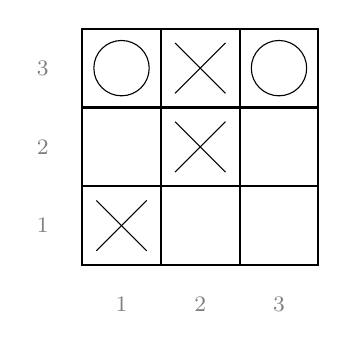
\begin{tikzpicture}
[thick]
  \foreach \x in {1,2,3}
    \foreach \y in {1,2,3}
    {
      \draw (\x,\y) +(-.5,-.5) rectangle ++(.5,.5);
    }

  %\draw (1,3) node{\begin{footnotesize}\textcolor{black!50}{1,3}\end{footnotesize}};
  %\draw (3,1) node{\begin{footnotesize}\textcolor{black!50}{3,1}\end{footnotesize}};
  \draw (0,3) node{\begin{footnotesize}\textcolor{black!50}{3}\end{footnotesize}};
  \draw (0,2) node{\begin{footnotesize}\textcolor{black!50}{2}\end{footnotesize}};
  \draw (0,1) node{\begin{footnotesize}\textcolor{black!50}{1}\end{footnotesize}};
  \draw (3,0) node{\begin{footnotesize}\textcolor{black!50}{3}\end{footnotesize}};
  \draw (2,0) node{\begin{footnotesize}\textcolor{black!50}{2}\end{footnotesize}};
  \draw (1,0) node{\begin{footnotesize}\textcolor{black!50}{1}\end{footnotesize}};

  \draw (2,3) node{\tikz \draw (-.32,-.32) -- (.32,.32);};
  \draw (2,3) node{\tikz \draw (-.32,.32) -- (.32,-.32);};

  \draw (2,2) node{\tikz \draw (-.32,-.32) -- (.32,.32);};
  \draw (2,2) node{\tikz \draw (-.32,.32) -- (.32,-.32);};

  \draw (1,1) node{\tikz \draw (-.32,-.32) -- (.32,.32);};
  \draw (1,1) node{\tikz \draw (-.32,.32) -- (.32,-.32);};

  \draw (1,3) node{\tikz \draw (0,0) circle (10pt);};

  \draw (3,3) node{\tikz \draw (0,0) circle (10pt);};
\end{tikzpicture}
\caption{A Tic-tac-toe board position, in which it is the ``circles'' player's turn to play. The labeling explains the indexing (left to right, bottom to top, starting at 1) of the grid.}
\label{fig:TTT}
\end{center}
\end{figure}

\begin{figure}
%%%\hspace{-0.8cm}
\begin{center}
\begin{tikzpicture}
    [thick,
level 1/.style={sibling distance=42mm},
level 2/.style={sibling distance=14mm},
level 3/.style={sibling distance=7mm}
]
\begin{footnotesize}
  \node[ellipse,draw] {Fig.~\ref{fig:TTT} state}
    child {node[rectangle,draw] {-1}
      child {node[circle,draw] {-1}
          edge from parent node[pos=0.5,fill=black!20] {2,1}
        }
      child {node[circle,draw] {0}
          child {node[rectangle,draw] {0}
              child {node[circle,draw] {0}
                edge from parent node[pos=0.5,fill=black!20] {3,2}}
              edge from parent node[pos=0.5,left,fill=black!20] {2,1}
            }
          child {node[rectangle,draw] {-1}
              child {node[circle,draw] {-1}
                edge from parent node[pos=0.5,fill=black!20] {2,1}}
              edge from parent node[pos=0.5,fill=black!20] {3,2}
            }
          edge from parent node[pos=0.5,fill=black!20] {3,1}
        }
      child {node[circle,draw] {0}
          child {node[rectangle,draw] {0}
              child {node[circle,draw] {0}
                edge from parent node[pos=0.5,fill=black!20] {3,1}}
              edge from parent node[pos=0.5,left,fill=black!20] {2,1}
            }
          child {node[rectangle,draw] {-1}
              child {node[circle,draw] {-1}
                edge from parent node[pos=0.5,fill=black!20] {2,1}}
              edge from parent node[pos=0.5,fill=black!20] {3,1}
            }
          edge from parent node[pos=0.5,fill=black!20] {3,2}
        }
      edge from parent node[pos=0.5,fill=black!20] {1,2}
    }
    child {node[rectangle,draw] {0}
      child {node[circle,draw] {0}
          child {node[rectangle,draw] {-1}
              child {node[circle,draw] {-1}
                edge from parent node[pos=0.5,fill=black!20] {3,2}}
              edge from parent node[pos=0.5,left,fill=black!20] {3,1}
            }
          child {node[rectangle,draw] {0}
              child {node[circle,draw] {0}
                edge from parent node[pos=0.5,fill=black!20] {3,1}}
              edge from parent node[pos=0.5,fill=black!20] {3,2}
            }
          edge from parent node[pos=0.5,fill=black!20] {1,2}
        }
      child {node[circle,draw] {0}
          child {node[rectangle,draw] {0}
              child {node[circle,draw] {0}
                edge from parent node[pos=0.5,fill=black!20] {3,2}}
              edge from parent node[pos=0.5,left,fill=black!20] {1,2}
            }
          child {node[rectangle,draw] {0}
              child {node[circle,draw] {0}
                edge from parent node[pos=0.5,fill=black!20] {1,2}}
              edge from parent node[pos=0.5,fill=black!20] {3,2}
            }
          edge from parent node[pos=0.5,fill=black!20] {3,1}
        }
      child {node[circle,draw] {0}
          child {node[rectangle,draw] {-1}
              child {node[circle,draw] {-1}
                edge from parent node[pos=0.5,fill=black!20] {3,1}}
              edge from parent node[pos=0.5,left,fill=black!20] {1,2}
            }
          child {node[rectangle,draw] {0}
              child {node[circle,draw] {0}
                edge from parent node[pos=0.5,fill=black!20] {1,2}}
              edge from parent node[pos=0.5,fill=black!20] {3,1}
            }
          edge from parent node[pos=0.5,fill=black!20] {3,2}
        }
      edge from parent node[pos=0.5,fill=black!20] {2,1}
    }
    child {node[rectangle,draw] {-1}
      child {node[circle,draw] {1}
          child {node[rectangle,draw] {-1}
              child {node[circle,draw] {-1}
                edge from parent node[pos=0.5,fill=black!20] {3,2}}
              edge from parent node[pos=0.5,left,fill=black!20] {2,1}
            }
          child {node[rectangle,draw] {1}
              edge from parent node[pos=0.5,fill=black!20] {3,2}
            }
          edge from parent node[pos=0.5,fill=black!20] {1,2}
        }
      child {node[circle,draw] {-1}
          edge from parent node[pos=0.5,fill=black!20] {2,1}
        }
      child {node[circle,draw] {-1}
          child {node[rectangle,draw] {-1}
              child {node[circle,draw] {-1}
                edge from parent node[pos=0.5,fill=black!20] {2,1}}
              edge from parent node[pos=0.5,left,fill=black!20] {1,2}
            }
          child {node[rectangle,draw] {-1}
              child {node[circle,draw] {-1}
                edge from parent node[pos=0.5,fill=black!20] {1,2}}
              edge from parent node[pos=0.5,fill=black!20] {2,1}
            }
          edge from parent node[pos=0.5,fill=black!20] {3,2}
        }
      edge from parent node[pos=0.5,fill=black!20] {3,1}
    }
    child {node[rectangle,draw] {-1}
      child {node[circle,draw] {1}
          child {node[rectangle,draw] {0}
              child {node[circle,draw] {0}
                edge from parent node[pos=0.5,fill=black!20] {3,1}}
              edge from parent node[pos=0.5,left,fill=black!20] {2,1}
            }
          child {node[rectangle,draw] {1}
              edge from parent node[pos=0.5,fill=black!20] {3,1}
            }
          edge from parent node[pos=0.5,fill=black!20] {1,2}
        }
      child {node[circle,draw] {-1}
          edge from parent node[pos=0.5,fill=black!20] {2,1}
        }
      child {node[circle,draw] {0}
          child {node[rectangle,draw] {-1}
              child {node[circle,draw] {-1}
                edge from parent node[pos=0.5,fill=black!20] {2,1}}
              edge from parent node[pos=0.5,left,fill=black!20] {1,2}
            }
          child {node[rectangle,draw] {0}
              child {node[circle,draw] {0}
                edge from parent node[pos=0.5,fill=black!20] {1,2}}
              edge from parent node[pos=0.5,fill=black!20] {2,1}
            }
          edge from parent node[pos=0.5,fill=black!20] {3,1}
        }
      edge from parent node[pos=0.5,fill=black!20] {3,2}
    };
\end{footnotesize}
\end{tikzpicture}
\end{center}
\caption{Minimax tree with initial position at Fig.~\ref{fig:TTT} state, \textbf{nodes} are states and \textbf{edges} are transitions, labeled with the move. Leafs are end-game states: 1 point for the win and -1 for the loss. Player is ``circles'' and plays first (first edges are player's moves).}
\label{fig:minimaxTTT}
\end{figure}
\subsection{Checkers, Alpha-beta}
Checkers, Chess and Go are also zero sum, \newglossaryentry{perfectinformation}{name={perfect-information},description={(game) in which all the players have complete knowledge of the (board) state of the game}}\glos{perfectinformation}, \newglossaryentry{partisan}{name={partisan},description={(game) which is not impartial, in which a player can do actions another can not do (move a faction while the other player(s) cannot)}}\glos{partisan}, deterministic strategy game. Theoretically, they all can be solved by exhaustive Minimax. 
In practice though, it is often intractable: their bounded versions are at least in \textsc{pspace} and their unbounded versions are \textsc{exptime}-hard \citep{GPC}. We can see the complexity of Minimax as $O(b^d)$ with $b$ the average branching factor of the tree (to search) and $d$ the average length (depth) of the game. 
For Checkers $b \approxeq 8$, but taking pieces is mandatory, resulting in a mean adjusted branching factor of $\approxeq 4$, while the mean game length is 70 resulting in a game tree complexity of $\approxeq 10^{31}$ \citep{allis1994}. It is already too large to have been solved by Minimax alone (on current hardware). From 1989 to 2007, there were artificial intelligences competitions on Checkers, all using at least alpha-beta pruning: a technique to make efficient cuts in the Minimax search tree while not losing optimality. 
The state space complexity of Checkers is the smallest of the 3 above-mentioned games with $\approxeq 5.10^{20}$ legal possible positions (conformations of pieces which can happen in games). As a matter of fact, Checkers have been (weakly) solved, which means it was solved for perfect perfect play on both sides (and always ends in a draw) \citep{Schaeffer07}. Not all positions resulting from imperfect play have been analyzed. 

Alpha-beta pruning (see Algorithm~\ref{alg:alphabeta}) is a branch-and-bound algorithm which can reduce Minimax search down to a $O(b^{d/2})=O(\sqrt{b^d})$ complexity if the best nodes are searched first ($O(b^{3d/4})$ for a random ordering of nodes). $\alpha$ is the maximum score than we (the maximizing player) are assured to get given what we already evaluated, while $\beta$ is the minimum score than the minimizing player is assured to get. When evaluating more and more nodes, we can only get a better estimate and so $\alpha$ can only increase while $\beta$ can only decrease. %If we find a node for us with an expected value below $\alpha$, we do not have to consider its subtree because it's sub-optimal play. If we find an expected value above $\beta$, it's sub-optimal play for the opponent. 
\begin{algorithm}
\caption{Alpha-beta algorithm}
\label{alg:alphabeta}
\begin{algorithmic}
\Function{alphabeta}{node,depth,$\alpha$,$\beta$,player}
    \If{$depth \leq 0$}
        \State \Return $value(player)$
    \EndIf
    \If{$player == us$}
        \ForAll{possible moves}
            \State $\alpha \gets \max{(\alpha, alphabeta(child,depth-1,\alpha,\beta,opponent))}$
            \If{$\beta \leq \alpha$}
                \State \textbf{break}
            \EndIf
        \EndFor
        \State \Return $\alpha$
    \Else
        \ForAll{possible moves}
            \State $\beta \gets \min{(\beta, alphabeta(child,depth-1,\alpha,\beta,us))}$
            \If{$\beta \leq \alpha$}
                \State \textbf{break}
            \EndIf
        \EndFor
        \State \Return $\beta$
    \EndIf
\EndFunction
\end{algorithmic}
\end{algorithm}
If we find a node for which $\beta$ becomes less than $\alpha$, it means that this position results from sub-optimal play. When it is because of an update of $\beta$, the sub-optimal play is on the side of the maximizing player (his $\alpha$ is not high enough to be optimal and/or the minimizing player has a winning move faster in the current sub-tree) and this situation is called an $\alpha$ cut-off. On the contrary, when the cut results from an update of $\alpha$, it is called a $\beta$ cut-off and means that the minimizing player would have to play sub-optimally to get into this sub-tree. When Starting the game, $\alpha$ is initialized to $-\infty$ and $\beta$ to $+\infty$. A worked example is given on Figure~\ref{fig:alphabeta}.
\tikzset{
alphacut/.style={postaction={decorate},
        decoration={markings,mark=at position .50 with {\draw (0.05,-.28)--(0.05,.28);\draw (-.05,-.28)--(-.05,.28);\node[right]{$\ \ \alpha \ cut$};}}},
betacut/.style={postaction={decorate},
        decoration={markings,mark=at position .50 with {\draw (0.05,-.28)--(0.05,.28);\draw (-.05,-.28)--(-.05,.28);\node[right]{$\ \ \beta \ cut$};}}},
}
\begin{figure}
%%%\hspace{-0.8cm}
\begin{center}
\begin{tikzpicture}
    [thick,
level 1/.style={sibling distance=32mm},
level 2/.style={sibling distance=14mm},
level 3/.style={sibling distance=7mm}
]
\begin{small}
  \node[circle,draw] (top) {3}
    child {node[rectangle,draw] (a) {3}
        child {node[circle,draw] (d3) {3}
            child {node[rectangle,draw] (d4) {2}}
            child {node[rectangle,draw] {3}}
        }
        child {node[circle,draw] (A) {}
            child {node[rectangle,draw] {5}}
            child {node[rectangle,draw] {} edge from parent[betacut]}
        }
    }
    child {node[rectangle,draw] (b) {0}
        child {node[circle,draw] {0}
            child {node[rectangle,draw] {0}}
        }
        child {node[circle,draw] (B) {}
            child {node[rectangle,draw] {}}
            child {node[rectangle,draw] {}}
            edge from parent[alphacut]
        }
    }
    child {node[rectangle,draw] (c) {2}
        child {node[circle,draw] {2}
            child {node[rectangle,draw] {2}}
            child {node[rectangle,draw] {1}}
        }
        child {node[circle,draw] {}
            child {node[rectangle,draw] {}}
            child {node[rectangle,draw] {}}
            edge from parent[alphacut]
        }
    };
    \node [blue,left] at (top.west) (d1) {$\alpha = 3$};
    \node [blue,left] at (a.west) (d2) {$\beta = 3$};
    \node [blue,left] at (b.west) {$\beta = 0$};
    \node [blue,left] at (c.west) {$\beta = 2$};
    \node [right] at (A.east) {$A$};
    \node [right] at (b.east) {$B$};
    \node [right] at (c.east) {$C$};
    \node [left,align=flush left] at (d1.west) {\textsc{Max}\ \ \ };
    \node [left,align=flush left] at (d2.west) {\textsc{Min}\ \ \ };
    \node [left] at (d3.west) {\textsc{Max}\ \ \ };
    \node [left] at (d4.west) {\textsc{Min}\ \ \ };
\end{small}
\end{tikzpicture}
\end{center}
\caption{Alpha-beta cuts on a Minimax tree, \textbf{nodes} are states and \textbf{edges} are transitions, labeled with the values of positions at the bottom (max depth). Here is the trace of the algorithm: \textbf{1.} descend leftmost first and evaluated 2 and 3, \textbf{2.} percolate max(2,3) higher up to set $\beta = 3$, \textbf{3.} $\beta$-cut in $A$ because its value is at least 5 (which is superior to $\beta=3$), \textbf{4.} Update of $\alpha=3$ at the top node, \textbf{5.} $\alpha$-cut in $B$ because it is at most 0 (which is inferior to $\alpha=3$), \textbf{6.} $\alpha$-cut in $C$ because it is at most 2, \textbf{7.} conclude the best value for the top node is 3.}
\label{fig:alphabeta}
\end{figure}
%Prior to Checkers being solved (meaning that we have a database of which moves to play for all positions resulting from optimal play), or if playing against a sub-optimal opponent, 
Alpha-beta is going to be helpful to search much deeper than Minimax in the same allowed time. The best Checkers program (since the 90s), which is also the project which solved Checkers \citep{SchaefferBBKMLLS07}, Chinook, has openings and end-game (for lest than eight pieces of fewer) books, and for the mid-game (when there are more possible moves) relies on a deep search algorithm. So, appart for the beginning and the ending of the game, for which it plays by looking up a database, it used a search algorithm. As Minimax and Alpha-beta are depth first search heuristics, all programs which have to answer in a fixed limit of time use \textit{iterative deepening}, a technique which consists in fixing limited depth which will be considered maximal and evaluating this position. As it does not relies in winning moves at the bottom, because the search space is too big in $branching^{depth}$, we need moves evaluation heuristics. We then iterate on growing the maximal depth for which we consider moves, but we are at least sure to have a move to play in a short time (at least the greedy depth 1 found move).

\subsection{Chess, Heuristics}
With a branching factor of $\approxeq 35$ and an average game length of 80 moves \citep{Shannon_1950}, the average game-tree complexity of chess is $35^{80}\approxeq 3.10^{123}$. \citet{Shannon_1950} also estimated the number of possible (legal) positions to be of the order of $10^{43}$, which is called the Shannon number. Chess AI needed a little more than just Alpha-beta to win against top human players (not that Checkers could not benefit it), particularly on 1996 hardware (first win of a computer against a reigning world champion, Deep Blue vs. Garry Kasparov). Once an AI has openings and ending books (databases to look-up for classical moves), how can we search deeper during the game, or how can we evaluate better a situation? In iterative deepening Alpha-beta (or other search algorithms like Negascout \citep{reinfeld1983negascout} or MTD-f\citep{Plaat1996}), one needs to know the value of a move at the maximal depth. If it does not correspond to the end of the game, there is a need for a evaluation heuristic. Some may be straight forward, like the resulting value of an exchange in pieces points. But some strategies sacrifice a queen in favor of a more advantageous tactical position or a checkmate, so evaluation heuristics need to take tactical positions into account. In Deep Blue, the evaluation function had 8000 cases, with 4000 positions in the openings book, all learned from 700,000 grandmaster games \citep{DeepBlue}. Nowadays, Chess programs are better than deep blue and generally also search less positions. For instance, Pocket Fritz (HIARCS engine) beats current grandmasters \citep{CitationNeeded} while evaluating 20,000 positions per second (740 MIPS on a smartphone) against Deep Blue's (11.38 GFlops) 200 millions per second.

\subsection{Go, Monte-Carlo Tree Search}
With an estimated number of legal 19x19 Go positions of $2.081681994 * 10^{170}$ \citep{tromp2006} (1.196\% of possible positions), and an average branching factor above Chess for \newglossaryentry{goban}{name=goban,description={board used for the game of Go},plural=gobans}\gloss{goban} from 9x9 and above, Go sets another limit for AI. For 19x19 gobans, the game tree complexity is up to $10^{360}$ \citep{allis1994}. Approaches other than systematic exploration of the game tree are required. One of them is Monte Carlo Tree Search \newglossaryentry{MCTS}{name=MCTS,description={Monte-Carlo Tree Search}}(\glos{MCTS}). Its principle is to randomly sample which nodes to expand and which to exploit in the search tree, instead of systematically expanding the build tree as in Minimax. For a given $node$ in the search tree, we note $Q(node)$ the sum of the simulations rewards on all the runs through $node$, and $N(node)$ the visits count of $node$. Algorithm~\ref{alg:mcts} details the MCTS algorithm and Fig.~\ref{fig:MCTS} explains the principle.

\begin{algorithm}
\caption{Monte-Carlo Tree Search algorithm. 
\textsc{ExpandFrom}$(node)$ is the tree (growing) policy function on how to select where to search from situation $node$ (exploration or exploitation?) and how to expand the game tree (deep-first, breadth-first, heuristics?) in case of untried actions. \textsc{Evaluate}$(tree)$ may have 2 behaviors: \textbf{1.} if $tree$ is complete (terminal), it gives an evaluation according to games rules, \textbf{2.} if $tree$ is incomplete, it has to give an estimation, either through simulation (for instance play at random) or an heuristic. \textsc{BestChild} picks the action that leads to the better value/reward from $node$. \textsc{Merge}$(node, tree)$ changes the existing tree (with $node$) to take all the $Q(\nu) \forall \nu \in tree$ (new) values into account. If $tree$ contains new nodes (there were some exploration), they are added to $node$ at the right positions.}
\label{alg:mcts}
\begin{algorithmic}
\Function{MCTS}{$node$}
    \While{computational time left}
        \State $tree \gets$ \textsc{ExpandFrom}$(node)$
        \State $tree.values \gets$ \textsc{Evaluate}$(tree)$
        \State \textsc{Merge}$(node, tree)$
    \EndWhile
    \State \Return \textsc{BestChild}$(node)$
\EndFunction
\end{algorithmic}
\end{algorithm}


The MoGo team \citep{GellyUCT, Gelly2006} introduced Upper Confidence Bounds for Trees (\newglossaryentry{UCT}{name=UCT,description={Upper Confidence Bounds for Trees}}\glos{UCT}) for \glos{MCTS} in Go AI. MoGo became the best 9x9 and 13x13 Go program, and the first to win against a pro on 9x9. UCT specializes MCTS in that it specifies \textsc{ExpandFrom} (as in Algorithm.~\ref{alg:expandfrom}) tree policy with a specific exploration-exploitation trade-off. UCB1 \citep{BanditBased} views the tree policy as a multi-armed bandit problem and so \textsc{ExpandFrom}$(node)$ UCB1 chooses the arms with the best upper confidence bound: $$\argmax_{c \in node.children} \frac{Q(c)}{N(c)}+k\sqrt{\frac{\ln N(node)}{N(c)}}$$ in which $k$ fixes the exploration-exploitation trade-off: $\frac{Q(c)}{N(c)}$ is simply the average reward when going through $c$ so we have exploitation only for $k=0$ and exploration only for $k=\infty$.

\citet{BanditBased} showed that the probability of selecting sub-optimal actions converges to zero and so that UCT MCTS converges to the minimax tree and so is optimal. Empirically, they found several convergences rates of UCT to be in $O(b^{d/2})$, as fast as Alpha-beta tree search, and able to deal with larger problems (with some error). For a broader survey on MCTS methods, see \citep{MCTSsurvey}.

\begin{algorithm}
\caption{UCB1 \textsc{ExpandFrom}}
\label{alg:expandfrom}
\begin{algorithmic}
\Function{ExpandFrom}{$node$}
    \If{$node$ is terminal}
        \State \Return $node$ \ \ \ \ \texttt{// terminal}
    \EndIf
    \If{$\exists c \in node.children\ s.t.\ N(c)=0 $}
        \State \Return $c$ \ \ \ \ \texttt{// grow}
    \EndIf
    \State \Return \textsc{ExpandFrom}$(\argmax_{c \in node.children)} \frac{Q(c)}{N(c)}+k\sqrt{\frac{\ln N(node)}{N(c)}})$ \ \ \ \ \texttt{// select}
\EndFunction 
\end{algorithmic}
\end{algorithm}

\begin{figure}
\begin{center}
\tikzset{
%/.style={postaction={decorate},
%        decoration={markings,mark=at position .50 with {\draw (0.05,-.28)--(0.05,.28);\draw (-.05,-.28)--(-.05,.28);\node[right]{$\ \ \beta \ cut$};}}},
}
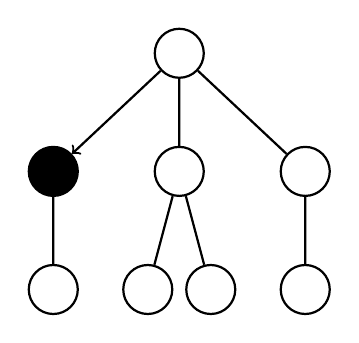
\begin{tikzpicture}
[
thick,
level 1/.style={sibling distance=16mm},
level 2/.style={sibling distance=8mm}
]
\begin{footnotesize}
  \node[circle,draw,inner sep=2.2mm] {}
    child {node[circle,draw,inner sep=2.2mm,fill] {} edge from parent [->]
        child {node[circle,draw,inner sep=2.2mm] {} edge from parent [-]}
        %child {node[circle,draw] {}}
    }
    child {node[circle,draw,inner sep=2.2mm] {}
        child {node[circle,draw,inner sep=2.2mm] {}
        }
        child {node[circle,draw,inner sep=2.2mm] {}
        }
    }
    child {node[circle,draw,inner sep=2.2mm] {}
        child {node[circle,draw,inner sep=2.2mm] {}
        }
    };
\end{footnotesize}
\end{tikzpicture}
\hspace{1cm}
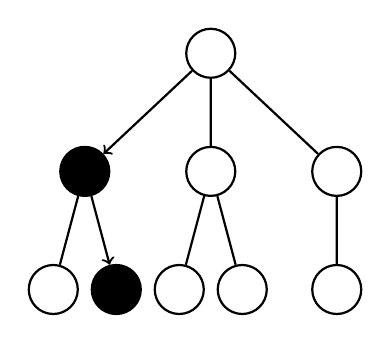
\begin{tikzpicture}
[
thick,
level 1/.style={sibling distance=16mm},
level 2/.style={sibling distance=8mm}
]
\begin{footnotesize}
  \node[circle,draw,inner sep=2.2mm] {}
    child {node[circle,draw,inner sep=2.2mm,fill] {} edge from parent [->]
        child {node[circle,draw,inner sep=2.2mm] {} edge from parent [-]}
        child {node[circle,draw,inner sep=2.2mm,fill] {} edge from parent [->]}
        %child {node[circle,draw,inner sep=2.2mm] {}}
    }
    child {node[circle,draw,inner sep=2.2mm] {}
        child {node[circle,draw,inner sep=2.2mm] {}
        }
        child {node[circle,draw,inner sep=2.2mm] {}
        }
    }
    child {node[circle,draw,inner sep=2.2mm] {}
        child {node[circle,draw,inner sep=2.2mm] {}
        }
    };
\end{footnotesize}
\end{tikzpicture}
\hspace{1cm}
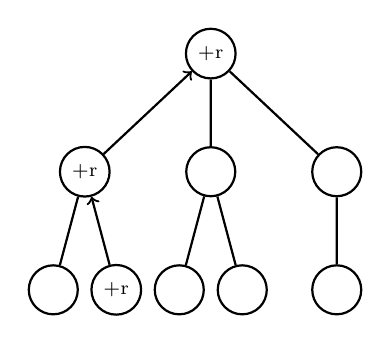
\begin{tikzpicture}
[
thick,
level 1/.style={sibling distance=16mm},
level 2/.style={sibling distance=8mm}
]
\begin{scriptsize}
  \node[circle,draw] {+r}
    child {node[circle,draw] {+r} edge from parent [<-]
        child {node[circle,draw,inner sep=2.2mm] {} edge from parent [-]}
        child {node[circle,draw] {+r} edge from parent [<-]}
        %child {node[circle,draw] {}}
    }
    child {node[circle,draw,inner sep=2.2mm] {}
        child {node[circle,draw,inner sep=2.2mm] {}
        }
        child {node[circle,draw,inner sep=2.2mm] {}
        }
    }
    child {node[circle,draw,inner sep=2.2mm] {}
        child {node[circle,draw,inner sep=2.2mm] {}
        }
    };
\end{scriptsize}
\end{tikzpicture}
\caption{An iteration of the \textbf{while} loop in MCTS, from left to right:
\textsc{ExpandFrom} select, \textsc{ExpandFrom} grow, \textsc{Evaluate} \& \textsc{Merge}.}
\label{fig:MCTS}
\end{center}
\end{figure}

With Go, we see clearly that humans do not play abstract strategy games using the same approach. Top Go players can reason about their opponent's move, but they seem to be able to do it in a qualitative manner, at another scale. So, while tree search algorithms help a lot for tactical play in Go, particularly by integrating openings/ending knowledge, pattern macthing algorithms are not yet at the strategical level of human players. When a MCTS algorithm learns something, it stays at the level of possible actions (even considering \newglossaryentry{positionalhashing}{name={positional hashing},description={a method for determining similarities in (board) positions using hash functions}}\glos{positionalhashing}), while the human player seems to be able to generalize, and re-use heuristics learned at another level.

%%%%%%%%%%%%%%%%%%%%%%%%%%%%%%%%%%%%%%%%%%%%%%%%%%%%%%%%%%%%%%%%%% 

\section{Games with Uncertainty}
An exhaustive list of games or even of games genres is beyond the scope/range of this thesis. %On the other hand, we will explain games for which randomness or incomplete information plays a key role with not-so-basic examples. 
All uncertainty boils down to incompleteness of information, being it the physics of the dice being thrown or the inability to measure what is happening in the opponent's brain. However,  we will speak of 2 types (sources) of uncertainty: extensional uncertainty, which is due to incompleteness in direct, measurable information, and intentional uncertainty, which is related to randomness in the game or in (the opponent's) decisions. As extreme illustrations of this: an agent acting without sending is under full extensional uncertainty, while an agent whose acts are the results of a perfect random generator is under full intentional uncertainty. The uncertainty coming from the opponent's mind/cognition lies in between, depending on the simplicity to model the game as an optimization procedure. The harder the game is to model, the harder it is to model the trains of thoughts our opponents can follow.

\subsection{Monopoly}
In Monopoly, there is few hidden information (\textit{Chance} and \textit{Community Chest} cards only), but there is randomness in the throwing of dice\footnote{Note that the sum of two uniform distributions is not a uniform but a Irwin-Hall, $\forall n>1, P([\sum_{i=1}^n{(X_i\in U(0,1))}]=x) \propto \frac{1}{(n-1)!}\sum_{k=0}^n(-1)^k{n\choose k}\max{((x-k)^{n-1},0)}$, converging towards a Gaussian (central limit theorem).}, and a substantial influence of the player's knowledge of the game. A very basic playing strategy would be to just look at the ruturn on investment (ROI) with regard to prices, rents and frequencies, choosing only based on the money you have and the possible actions of buying or not. A less naive way to play should evaluate the questions of buying with regard to what we already own, what others own, our cash and advancement in the game. The complete state space is huge (places for each players $\times$ their money $\times$ their possessions), but according to \cite{MonopolyMarkov}, we can model the game for one player (as he has no influence on the dice rolls and decisions of others) as a Markov process on 120 ordered pairs: 40 board spaces $\times$ possible number of doubles rolled so far in this turn (0, 1, 2). With this model, it is possible to compute more than simple ROI and derive applicable and interesting strategies. So, even in monopoly, which is not lottery playing or simple dice throwing, a simple probabilistic modeling yields a robust strategy. Additionally, \cite{MonopolyFrayn05} used genetic algorithms to generate the most efficient strategies for portfolio management. %We observe that the main difficulty of Monopoly: randomness in a gameplay in which we have to make up a strategy, can be dealt with with probabilistic modeling. 

Monopoly is an example of a game in which we have complete direct information about the state of the game, intentional uncertainty due to the roll of the dice (randomness) can be dealt with thanks to probabilistic modeling (Markov processes here). The opponent's actions are relatively easy to model due to the fact that the goal is to maximize cash and that there are not many different efficient strategies (not many Nash equilibrium if it were a stricter game) to attain it. In general, the presence of chance does not invalidates previous (game theoretic / game trees) approaches but transforms exact computational techniques into stochastic ones: finite states machines become probabilistic Bayesian networks for instance.

%\subsection{Diplomacy}
%\subsection{Bridge}
\subsection{Battleship}
Battleship (also called ``naval combat'') is a guessing game generally played with two 10x10 grids for each players: one is the player's ships grid, and one is to remember/infer the opponent's ships positions. The goal is to guess where the enemy ships are and sink them by firing shots (torpedoes). There is \textbf{incompleteness} of information but no randomness. Incompleteness can be dealt with with probabilistic reasoning. The classic setup of the game consist in two ships of length 3 and one ship of each lengths of 2, 4 and 5; in this setup, there are 1,925,751,392 possible arrangements for the ships. The way to take advantage of all possible information is to update the probability that there is a ship for all the squares each time we have additional information. So for the 10x10 grid we have a 10x10 matrix $O_{1:10,1:10}$ with $O_{i,j} \in \{true,false\}$ being the $i$th row and $j$th column random variable of the case being occupied. With $ships$ being unsunk ships, we always have: $$\sum_{i,j}P(O_{i,j}=true) = \frac{\sum_{k\in ships}length(k)}{10 \times 10}$$ For instance for a ship of size 3 alone at the beginning we can have prior distributions on $O_{1:10,1:10}$ by looking at combinations of its placements (see Fig.~\ref{fig:battleship}). We can also have priors on where the opponent likes to place her ships. Then each round we will either hit or miss in $i,j$. When we hit, we know $P(O_{i,j}=true)=1.0$ and will have to revise the probabilities of surrounding areas, and everywhere if we learned the size of the ship, with possible placement of ships. If we did not sunk a ship, the probabilities of uncertain (not 0.0 or 1.0) positions around $i,j$ will be highered according to the sizes of remaining ships. If we miss, we know $P([O_{i,j}=false])=1.0$ and can also revise (lower) the surrounding probabilities, an example of that effect is shown in Fig.~\ref{fig:battleship}. 

Battleship is a game with few intensional uncertainty (no randomness), particularly because the goal quite strongly conditions the action (sink ships as fast as possible) but a large part of extensional uncertainty (incompleteness of direct information), which goes down rather quickly once we act, if we update a probabilistic model of the map/grid. If we compare Battleship to a variant in which we could see the adversary board, playing would be straightforward (just hit ships we know the position on the board), now in real Battleship we have to model our uncertainty due to the incompleteness of information, without even beginning to take into account the psychology of the opponent in placement as a prior. The cost of solving an imperfect information game increases greatly from its perfect information variant: it seems to be easier to model stochasticity (chance, a source of randomness) than to model a hidden (complex) system for which we only observe (indirect) effects.

\begin{figure}[h!]
\begin{center}
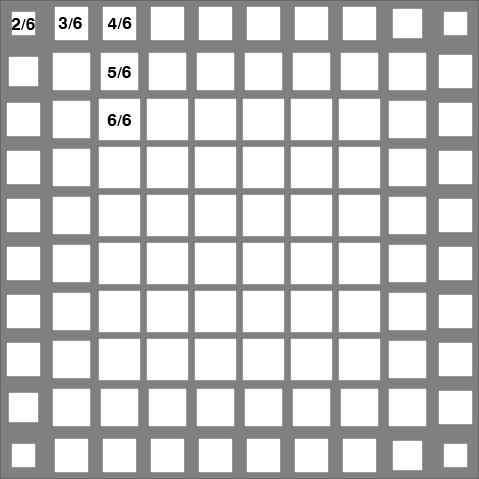
\includegraphics[width=7.8cm]{images/battleship_board_3_init_annotated.png} 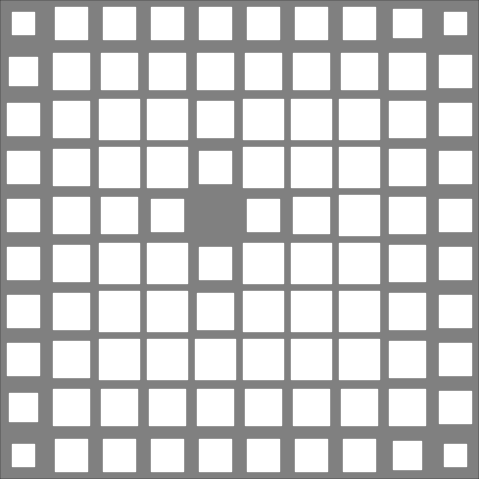
\includegraphics[width=7.8cm]{images/battleship_board_3_1miss.png}
\caption{Left: visualization of probabilities for squares to contain a ship of size 3 ($P(O_{i,j})=true$) initially, assuming uniform distribution of this type of ship. Annotations correspond to the \textit{number of combinations} (on six, the maximum number of conformations), Right: same probability after a miss in (5, 5). The larger the white area, the higher the probability.}
\label{fig:battleship}
\end{center}
\end{figure}


\subsection{Poker}
Poker\footnote{We deal mainly with the \textit{Limit Hold'em} variant of Poker.} is a zero-sum (without the house's cut), imperfect information and stochastic betting game. Poker ``AI'' is as old as game theory \citep{nash51a}, but the research effort for human-level Poker AI started in the end of the 90s. The interest for Poker AI is such that there are annual AAAI computer Poker competitions\footnote{\url{http://www.computerpokercompetition.org/}}. \citet{Billings98pokeras} defend Poker as an interesting game for decision-making research, %combining imperfect information with randomness. The
because the task of building a good/high level Poker AI (player) entails to take decisions with incomplete information about the state of the game, incomplete information about the opponents' intentions, and model their thoughts process to be able to bluff efficiently. A Bayesian network can combine these uncertainties and represent the player's hand, the opponents' hands and their playing behavior conditioned upon the hand, as in \citep{Korb99bayesianpoker}. A simple ``risk evaluating'' AI (folding and raising according to the outcomes of its hands) will not prevail against good human players. Bluffing, as described by \citet{VonNeumannMorgenstern1944} ``to create uncertainty in the opponent's mind'', is an element of Poker which needs its own modeling. \citet{Southey05bayesbluff} also give a Bayesian treatment to Poker, separating the uncertainty resulting from the game (draw of cards) and from the opponents' strategies, and focusing on bluff. From a game theoretic point of view, Poker is a \newglossaryentry{bayesiangame}{name={Bayesian game},description={a game in which information about knowledge about payoffs is incomplete}}\glos{bayesiangame}. In a Bayesian game, the normal form representation requires describing the strategy spaces, type spaces, payoff and belief functions for each player. It maps to all the possible game trees along with the agents' information state representing the probabilities of individual moves, called the extensive form. Both these forms scale very poorly (exponentially). \citet{Koller97representationsand} used the sequence form transformation, the set of realization weights of the sequences of moves\footnote{for a given player, a sequence is a path down the game tree isolating only moves under their control}, %of extensive form with informations sets,
to search over the space of randomized strategies for Bayesian games automatically. Unfortunately, strict game theoretic optimal strategies for full-scale Poker are still not tractable this way, two players Texas Hold'em having a state space $\approxeq O(10^{18})$. \citet{BillingsBDHSSS03} approximated the game-theoretic optimal strategies through abstraction and are able to beat strong human players (not world-class opponents).

Poker is a game with both extensional and intentional uncertainty, from the fact that the opponents' hands are hidden, the chance in the draw of the cards, the opponents' model about the game state and their model about our mental state(s) (leading our decision(s)). While the iterated reasoning (``if she does A, I can do B'') is (theoretically) finite in Chess due to perfect information, it is not the case in Poker (``I think she thinks I think...''). The combination of different sources of uncertainty (as in Poker) makes it complex to deal with it (somehow, the sources of uncertainty must be separated), and we will see that both these sources of uncertainties arise (at different levels) in video games.

%%%%%%%%%%%%%%%%%%%%%%%%%%%%%%%%%%%%%%%%%%%%%%%%%%%%%%%%%%%%%%%%%% 

\section{FPS}

\subsection{Gameplay and AI}
First person shooters \newglossaryentry{gameplay}{name=gameplay,description={describes the interactive aspects of game design, which constraints the players possible behaviors and the players' goals in a given game},plural=gameplays}\glos{gameplay} consist in controlling an agent in first person view, centered on the weapon, a gun for instance. The firsts FPS popular enough to bring the genre its name were Wolfeinstein 3D and Doom, by iD Software. Other classic FPS (series) include Duke Nukem 3D, Quake, Half-Life, Team Fortress, Counter-Strike, Unreal Tournament, Tribes, Halo, Medal of Honor, Call of Duty, Battlefield, etc. The distinction between ``fast FPS'' (e.g. Quake series, Unreal Tournament series) and others is made on the speed at which the player moves. In ``fast FPS'', the player is always jumping, running much faster and playing more in 3 dimensions than on discretely separate 2D ground planes. Game types include (but are not limited to):
\begin{itemize}
    \item single-player missions, depending of the game design.
    \item capture-the-flag (CTF), in which a player has to take the flag inside the enemy camp and bring it back in her own base.
    \item free-for-all (FFA), in which there are no alliances.
    \item team deathmatch (TD), in which two (or more) teams fight on score.
    \item various gather and escort (including hostage or payload modes), in which one team has to find and escort something/somebody to another location.
    \item duel/tournament/deathmatch, 1 vs 1 matches (mainly ``fast FPS'').
\end{itemize}
From these various game types, the player has to maximize its damage (or positive actions) output while staying alive. For that, she will navigate her avatar in an uncertain environment (partial information and other players intentions) and shoot (or not) at targets with specific weapons.

Some games allow for instant (or delayed, but asynchronous to other players) respawn (recreation/rebirth of a player), most likely in the ``fast FPS'' (Quake-like) games, while in others, the player has to wait for the end of the round to respawn. In some games, weapons, ammunitions, health, armor and items can be picked on the ground (mainly ``fast FPS''), in others, they are fixed at the start or can be bought in game (with points). The map design can make the gameplay vary a lot, between indoors, outdoors, arena-like or linear maps. According to maps and gameplay styles, combat may be well-prepared with ambushes, sniping, indirect (zone damages), or close proximity (even to fist weapons). Most often, there are strong tactical positions and effective ways to attack them. 

While ``skill'' (speed of the movements, accuracy of the shots) is easy to emulate for an AI, team-play is much harder for bots and it is always a key ability. Team-play is the combination of distributed evaluation of the situation, planning and distribution of specialized tasks. Very high skill also requires integrating over enemy's tactical plans and positions to be able to take indirect shots (grenades for instance) or better positioning (coming from their back), which is hard for AI too. An example of that is that very good human players consistently beat the best bots (nearing 100\% accuracy) in Quake III (which is an almost pure skill ``fast FPS''), because they take advantage of being seen just when their weapons reload or come from their back. Finally, bots which equal the humans by a higher accuracy are less fun to play with: it is a frustrating experience to be shot across the map, by a bot which was stuck in the door because it was pushed out of its trail.

\subsubsection{State of the art}

FPS AI consists in controlling an agent in a complex world: it can have to walk, run, crouch, jump, swim, interact with the environment and tools, and sometimes even fly. Additionally, it has to shoot at moving, coordinated and dangerous, targets. %The first solution, in Wolfeinstein 3D, was to have enemies just shoot or run towards the player. The game was basically a linear indoors two-dimensional (no jumps, no stairs, nor the possibility to shoot up or down) labyrinth. 
On a higher level, it may have to gather weapons, items or power-ups (health, armor, etc.), find interesting tactical locations, attack, chase, retreat...

The Quake III AI is a standard for Quake-like games \citep{waveren-02-artificial}. It consists in a layered architecture (hierarchical) FSM. At the sensory-motor level, it has an Area Awareness System (AAS) which detects collisions, accessibility and computes paths. The level above provides intelligence for chat, goals (locations to go to), goals and weapons selection through fuzzy logic. Higher up, there are the behavior FSM (``seek goals'', chase, retreat, fight, stand...) and production rules (if-then-else) for squad/team AI and orders. A team of bots always behaves following the orders of one of the bots. Bots have different natures and tempers, which can be accessed/felt by human players, specified by fuzzy relations on ``how much the bot wants to do, have, or use something''. A genetic algorithm was used to optimize the fuzzy logic parameters for specific purposes (like performance). This bot is fun to play against and is considered a success, however Quake-like games makes it easy to have high level bots because very good players have high accuracy (no fire spreading), so they do not feel cheated if bots have a high accuracy too. Also, the game is mainly indoors, which facilitates tactics and terrain reasoning. Finally, cooperative behaviors are not very evolved and consist in acting together towards a goal, not with specialized behaviors for each agent.

The more recent FPS games have dealt with these limitations by using combinations of STRIPS planning (F.E.A.R. \citep{orkinGDC_FEAR}), hierarchical task networks (HTN) (Killzone 2 \citep{Killzone2_HTN} and ArmA \citep{ArmA1_HTN}), Behavior trees (Halo 2 \citep{Isla}). Left4Dead (a cooperative PvE FPS) uses a global supervisor of the AI to set the pace of the threat to be the most enjoyable for the player \citep{left4dead2009}.% (Crysis2 BF3)
%\begin{color}{red}explain Behavior trees? \\
%\url{http://files.aigamedev.com/insiders/BehaviorTrees_Slides.pdf}\\ 
%\url{http://altdevblogaday.com/2011/02/24/introduction-to-behavior-trees/}\\
%\url{http://aigamedev.com/open/article/anatomy-ai-architecture/}\\
%\url{http://www.cgf-ai.com/docs/straatman_remco_killzone_ai.pdf} \end{color}

In research, \citet{Laird01} focused on learning rules for opponent modeling, planning and reactive planning (on Quake), so that the robot builds plan by anticipating the opponent's actions. \citet{LeHy04,theseRonan} used robotics inspired Bayesian models to quickly learn the parameters from human players (on Unreal Tournament). \citet{Zanetti2004} and \citet{westraQ3} applied evolutionary neural networks to optimize Quake III bots. Predicting opponents positions is a central task to believability and has been solved successfully using particle filters \citep{particlefiltergameAI} and other models (like Hidden Semi-Markov Models) \citep{Hladky_anevaluation}. Multi-objective neuro-evolution \citep{Zanetti2004,schrum_cig11competition} combines learning from human traces with evolutionary learning for the structure of the artificial neural network, and leads to realistic (human-like) behaviors, in the context of the BotPrize challenge (judged by humans) \citep{Hingston_2009}.

\subsubsection{Challenges}

Single-player FPS campaigns immersion could benefit from more realistic bots and clever squad tactics. Multi-player FPS are competitive games, and a better game AI should focus on:
\begin{itemize}
    \item \textbf{believability} requires the AI to take decisions with the same informations than the human player (fairness) and to be able to deal with unknown situation.
    \item \textbf{surprise} and {unpredictability} is key for both performance and the long-term interest in the human player in the AI.
    \item \textbf{performance}, to give a challenge to human players, can be achieved through cooperative, planned and specialized behaviors.
\end{itemize}

%%%%%%%%%%%%%%%%%%%%%%%%%%%%%%%%%%%%%%%%%%%%%%%%%%%%%%%%%%%%%%%%%% 

\section{(MMO)RPG}

\subsection{Gameplay and AI}
Inspired directly by tabletop and live action role-playing games (Dungeon \& Dragons) as new tools for the game masters, it is quite natural for the RPG to have ended up on computers. The firsts digital RPG were text (Wumpus) or ASCII-art (Rogue, NetHack) based. The gameplay evolved considerably with the technique. Nowadays, what we will call a role playing game (RPG) consist in the incarnation by the human player of an avatar (or a team of avatars) with a class: warrior, wizard, rogue, priest, etc., having different skills, spells, items, health points, stamina/energy/mana (magic energy) points. Generally, the story brings the player to solve puzzles and fight. In a fight, the player has to take decisions about what to do but plays a lesser role in performing the action than in a FPS game. In a FPS, she has to move the character (egocentrically) and aim to shoot; in a RPG, she has to position itself (often way less precisely and continually) and just decide which ability to use on which target (or a little more for ``action RPG''). Classic RPG include: Fallout, The Elders Scrolls (from Arena to Skyrim), Secret of Mana, Zelda, Final Fantasy, Diablo, Baldur's Gate. A MMORPG (e.g. World of Warcraft, AION or EVE Online) consist in a role-playing game in a persistent, multi-player world. There usually are players-run factions fighting each others’ (PvP) and players versus environment (PvE) situations. \\glos{PvE} may be a cooperative task in which human players fight together against different NPC, and in which the cooperation is at the center of the gameplay. PvP is also a cooperative task, but more policy and reactions-based than a trained and learned choregraphy as for PvE. We can distinguish three types (or modality) of NPC which have different game AI needs:
\begin{itemize}
    \item world/neutral/civilian NPC: gives quests, takes part in the world's or game's story, talks,
    \item ``mob''/hostile NPC that the player will fight, 
    \item ``pets''/allied NPC: acts by the players' sides.
    \item persistent character AI could maintain the players' avatars in the world when they are disconnected.
\end{itemize}
NPC acting strangely are sometimes worse for the player's immersion than immobile and dull ones. However, it is more fun for the player to battle with hostile NPC which are not too dumb or predictable. Players really expect allied NPC to at least not hinder them, and it is even better when they adapt to what the player is doing. %Finally, for MMORPG, persistent character AI could maintain the player's avatar in the world when she is enjoying real-life.

\subsubsection{State of the art}

Methods used in FPS are also used in RPG. The needs are sometimes a little different for RPG games, for instance RPG need interruptible behaviors, along with stronger story-telling capabilities, for which they use (logical) story representations (ontologies) \citep{kline2009,riedl11}. Behavior multi-queues \citep{Cutumisu09} resolve the problems of having resumable, collaborative, real-time and parallel behavior, and tested their approach on Neverwinter Nights. Basically they use prioritized behavior queues which can be inserted (for interruption and resumption) in each others. AI directors are control programs tuning the difficulty and pace of the game session in real-time from player's metrics. \citet{kline2011} used an AI director to adapt the difficulty of Dark Spore to the performance (interactions and score) of the player in real-time.

\subsubsection{Challenges}

There are mainly two axes for RPG games to bring more fun: interest in the game play(s), and immersion. For both these topics, we think game AI can bring a lot:
\begin{itemize}
    \item \textbf{believability} of the agents will come from AI approaches than can deal with new situations, being it because they were not dealt with during game development (because the ``possible situations'' space is too big) or because they were brought by the players' unforeseeable actions. Scripts and strict policies approaches will be in difficulty here. %, and we will assist to other Skyrim's NPC blunders.
    \item \textbf{interest} (as opposed to boredom) for the human players in the game style of the AI will come from approaches which can generate different behaviors in a given situation. Expectable AI particularly affects replayability negatively.
    \item \textbf{performance} relative to the gameplay will come from AI approaches than can fully deal with cooperative behavior. One solution is to design mobs to be orders of magnitude stronger (in term of hit points and damages) than players characters, or more numerous. Another, arguably more entertaining, solution is to bring the mobs behavior to a point where they are a challenge for the team of human players.
\end{itemize}
Both believability and performance require to deal with uncertainty of the game environment. RPG AI problem spaces are not tractable for a frontal (low-level) search approach nor are there few enough situations to consider to just write a bunch of script and puppeteer artificial agents at any time.

%%%%%%%%%%%%%%%%%%%%%%%%%%%%%%%%%%%%%%%%%%%%%%%%%%%%%%%%%%%%%%%%%% 

\section{RTS}
As RTS are the central focus on this thesis, we will discuss specific problems and solution more in depth in their dedicated chapters, simply brushing here the underlying major research problems.

\subsection{Gameplay and AI}
RTS gameplay consist in gathering resources, building up an economic and military power through growth and technology, to defeat your opponent by destroying his base, army and economy. It requires dealing with strategy, tactics, and units management (often called micro-management) in real-time. Strategy consist in what will be done in the long term as well as predicting what the enemy is doing. It particularly deals with the economy/army trade-off estimation, army composition, long-term planning. The three aggregate indicators for strategy are aggression, production, and technology. The tactical aspect of the gameplay is dominated by military moves: when, where (with regard to topography and weak points), how to attack or defend. This implies dealing with \textit{extensional} (what the invisible units under ``fog of war'' are doing) and \textit{intentional} (what will the visible enemy units do) uncertainty. Finally, at the actions/motor level, micro-management is the art of maximizing the effectiveness of the units \textit{i.e.} the damages given/damages received ratio. For instance: retreat and save a wounded unit so that the enemy units would have to chase it either boosts your firepower or weakens the opponent's. Both \citep{Human-LevelAIKillerApplication} and \cite{gunn} propose that RTS AI is one of the most challenging genres, because all levels in the hierarchy of decisions are of importance.
%%% incompleteness of information yielding uncertainty

In chronological order, RTS include (but are not limited to): Ancient Art of War, Herzog Zwei, Dune II, Warcraft, Command \& Conquer, Warcraft II, C\&C: Red Alert, Total Annihilation, Age of Empires, StarCraft, Age of Empires II, Tzar, Cossacks, Homeworld, Battle Realms, Ground Control, Spring Engine games, Warcraft III, Total War, Warhammer 40k, Sins of a Solar Empire, Supreme Commander, StarCraft II. 

XXX ???

\subsubsection{State of the art}
\citet{Buro04callfor} called for AI research in RTS games and identified the technical challenges as adversarial planning under uncertainty, learning and opponent modeling, and spatial and temporal reasoning.  

On planning under uncertainty, \citet{LTW} used \newacronym{cbr}{CBR}{case-based reasoning}\glos{cbr} to perform dynamic plan retrieval extracted from domain knowledge in Wargus (Warcraft II clone). \citet{Ontanon2007} based their real-time case-based planning (CBP) system on a plan dependency graph which is learned from human demonstration in Wargus. In \citep{Mishra2008,Ontanon2010,metalevelbehavioradaptrts}, they used a knowledge-based approach to perform situation assessment to use the right plan, and revise it (integrating learning, planning, and problem solving in CBR), performing runtime adaptation by monitoring its performance. \citet{Trusty2011} used a genetic-algorithm inspired method to mix and optimize existing expert plan, also in Wargus. \citet{Chung05} adapted Monte-Carlo tree search to planning in RTS games and applied it to a capture-the-flag mod of Open RTS. \citet{UCT} applied UCT (MCTS algorithm) to tactical assault planning in Wargus. Reactive planning and goal-driven autonomy (that is, find the more relevant goal to follow in unknown situations) are studied in \citep{Weber2010cr,WeberCIG10}. \citet{Churchill2011} used abstractions and heuristics to produce a real-time build-order planner. %\citet{CadenaG11} used fuzzy CBR for strategic and tactical planning.
%\citep{Weber2010qf}

On learning and opponent modeling, \citet{schadd2007opponent} used hierarchical classifiers to learn the opponent's behavior in Spring (an open source clone of Total Annihilation). \citet{HsiehS08} learned players' strategy models with CBR by mining replays of StarCraft. \citet{weberStrat} applied data-mining to StarCraft replays to learn to predict strategies. \citet{HagelbackCIG10} performed a study on what are the human like characteristics of play in RTS games. \citet{Kim2010} clusterized build-orders to learn them from replays. \citet{Kabanza2010} studied strategic and tactic plan and intent recognition by probabilistic weighting of plans from a plan library, on StarCraft. In \citep{SYNNAEVE:OpeningPred}, we clusterized replays to annotate them with openings (strategies) and then learned the parameters of a predictive Bayesian model for strategies from StarCraft replays. In \citep{SYNNAEVE:StratPred}, we also learned parameters of a strategy prediction Bayesian model from StarCraft replays but in an unsupervised fashion (predicting build/tech trees). \citet{HMMstrat_RTS_AIIDE11} also had an unsupervised learning approach by fitting HMM to players build actions (from StarCraft replays) and clustering the most probable HMM transitions to be subsets of strategies.

On spatial and temporal reasoning, \citet{Forbus2002} presented tactical qualitative description of terrain for wargames through geometric and pathfinding analysis. \citet{Perkins2010} automatically extracted choke points and regions of StarCraft maps from a pruned Voronoi diagram. \citet{Southey2007} infered ``complex agent motions from partial information'' using hidden semi-markov models including A* as a motion model. \citet{ButlerCIG10} applied forward and inverse models simulation to the prediction of units movements from partial observations onto a RTS. \citet{weber2011aiide} implemented a simpler particle filter for state estimation in StarCraft. \citet{SORTS} used a cognitive approach mimicking human attention for tactics and units control. \citet{Miles2007} and \citet{SmithCIG10} co-evolved influence map trees for spatial (tactical) reasoning in RTS games. \citet{IntelligentMoving} combined flocking \citep{Reynolds1987} with influence maps, while \citet{teamCompositionRTS} enhanced it, supporting team composition and maneuvering by learning a self-organizing map. \citet{Hagelback2009} presented a multi-agent potential field based bot and we presented a similar unifying Bayesian model for micro-management \citep{SYNNAEVE:Micro} in which units are attracted or repulsed by different real or virtual units or goals.
% \citet{NovaBot2011}

\subsubsection{Challenges}

In \citep{Buro04callfor}, the challenges of RTS AI are:
\begin{itemize}
    \item ``adversarial planning under uncertainty'', and for that abstractions have to be found both allowing to deal with partial observations and to plan in real-time.
    \item ``learning and opponent modeling'': adaptivity plays a key role in the strength of human players.
    \item ``spatial and temporal reasoning'': tactics using the terrain features and good timings are essential for higher level play.
\end{itemize}
To these challenges, we would like to add the difficulty of inter-connecting all special cases resolutions of these problems: both for collaborative (economical and logistical) management of the resources, and for sharing of uncertainty quantization in the decision-making processes. This will be extended further in the next chapters as RTS are the main focus of this thesis.

%%%%%%%%%%%%%%%%%%%%%%%%%%%%%%%%%%%%%%%%%%%%%%%%%%%%%%%%%%%%%%%%%% 

\section{Games Characteristics}
All the types of video games that we saw before require to deal with imperfect information and sometimes with randomness, while elaborating a strategy (possibly from underlying policies). From a game theoretic point of view, these video games are close to what is called a \glos{bayesiangame} \citep{osborne-rubinstein}. %%% Their formal description is:
%%% \begin{itemize}
%%% \item $N$, a finite set of players,
%%% \item $\Omega$, a finite set of states,
%%% \end{itemize}
%%% $$\forall \mathrm{player}\ i \in N$$
%%% \begin{itemize}
%%% \item $A_i$, a set of actions,
%%% \item $T_i$, a set of signals that can be observed by $i$,
%%% \item $p_i$, a probability measure on $\Omega$ (prior belief of $i$),
%%% \item $\succ_i$, a preference relation on the set of probability measures over $A\times \Omega$ with $A = \times_{j \in N}A_j$.
%%% \end{itemize}
However, solving Bayesian games is non-trivial, there are no generic and efficient approaches, and so it has not been done formally for card games with more than a few cards. \citet{BillingsBDHSSS03} approximated a game theoretic solution for Poker through abstraction heuristics, it leads to believe than game theory can be applied at the higher (strategic) abstracted levels of video games.

We do not pretend to do a complete taxonomy of video games and AI (e.g. \citep{gunn}), but we wish to provide all the major informations to differentiate game genres (gameplays). To grasp the challenges they pose, we will provide abstract measures of complexity.

\subsection{Combinatory}
``How does the state of possible actions grow?'' To measure this, we used a measure from perfect information zero-sum games (as Checkers, Chess and Go): the branching factor $b$ and the depth $d$ of a typical game. The complexity of a game (for taking a decision) is proportional to $b^d$. The average branching factor for a board game is easy to compute: it is the average number of possible moves for a given player. For Poker, we set $b=3$ for \textit{fold, check} and \textit{raise}. $d$ should then be defined over some time, the average number of events (decisions) per hour in Poker is between $20$ to $240$. For video-games, we defined $b$ to be the average number of possible moves at each decision, so for ``continuous'' or ``real-time'' games it is some kind of function of the useful discretization of the virtual world at hand. $d$ has to be defined as a frequency at which a player (artificial or not) has to take decisions to be competitive in the game, so we will give it in $d/time\_unit$. For instance, for a car (plane) racing game, $b \approxeq 50-500$ because $b$ is a combination of throttle ($\ddot{x}$) and direction ($\theta$) sampled values that are relevant for the game world, with $d/min$ at least $60$: a player needs to correct her trajectory \textit{at least} once a second. In RTS games, $b \approxeq 200$ is a lower bound (in StarCraft we may have between $50$ to $400$ units to control), and very good amateurs and professional players perform more than $300$ actions per minute.

The sheer size of $b$ and $d$ in video games make it seem intractable, but humans are able to play, and to play well. To explain this phenomenon, we introduce ``vertical'' and ``horizontal'' continuities in decision making. Fig.~\ref{fig:abstractdecisionhierarchy} shows how one can view the decision-making process in a video game: at different time scales, the player has to choose between strategies to follow, that can be realized with the help of different tactics. Finally, at the action/output/motor level, these tactics have to be implemented one way or the other. So, matching Fig.~\ref{fig:abstractdecisionhierarchy}, we could design a Bayesian model:
\begin{itemize}
\item $S^{t,t-1} \in {Attack,Defend,Collect,Hide}$, the strategy variable
\item $T^{t,t-1} \in {Front,Back,Hit-and-run,Infiltrate}$, the tactics variable
%\item $S^{t,t-1} \in {Attack,Defend,Seach,Hide}$, the strategy variable
%\item $T^{t,t-1} \in {Front,Back,Prepare,Rush}$, the tactics variable
\item $A^{t,t-1} \in {low\_level\_actions}$, the actions variable
\item $O_{1:n}^{t} \in \{observations\}$, the set of observations variables
\end{itemize}
%\begin{eqnarray*}
$$P(S^{t,t-1},T^{t,t-1},A^{t,t-1},O_{1:n}^t) = P(S^{t-1}).P(T^{t-1}).P(A^{t-1})$$
$$.P(O_{1:n}^t).P(S^t|S^{t-1},O_{1:n}^t).P(T^t|S^t,T^{t-1},O_{1:n}^t).P(A^t|T^t,A^{t-1},O_{1:n}^t)$$
\begin{itemize}
    \item $P(S^t|S^{t-1},O_{1:n}^t)$ should be read as ``the probability distribution on the strategies at time $t$ is determined/influenced by the distribution on the strategies at time $t-1$ and (all) the distributions on the observations at time $t$''.
    \item $P(T^t|S^t,T^{t-1},O_{1:n}^t)$ should be read as ``the probability distribution on the tactics at time $t$ is determined by the distribution on the strategies at time $t$, the distribution on the tactics at time $t-1$ and the distributions on the observations at time $t$''.
    \item $P(A^t|T^t,A^{t-1},O_{1:n}^t)$ should be read as ``the probability distribution on the actions at time $t$ is determined by the distribution on the tactics at time $t$, the distribution on the actions at time $t-1$ and the distributions on the observations at time $t$''.
\end{itemize}
%\end{eqnarray*}

\begin{figure}
%%%\hspace{-0.8cm}
\begin{center}
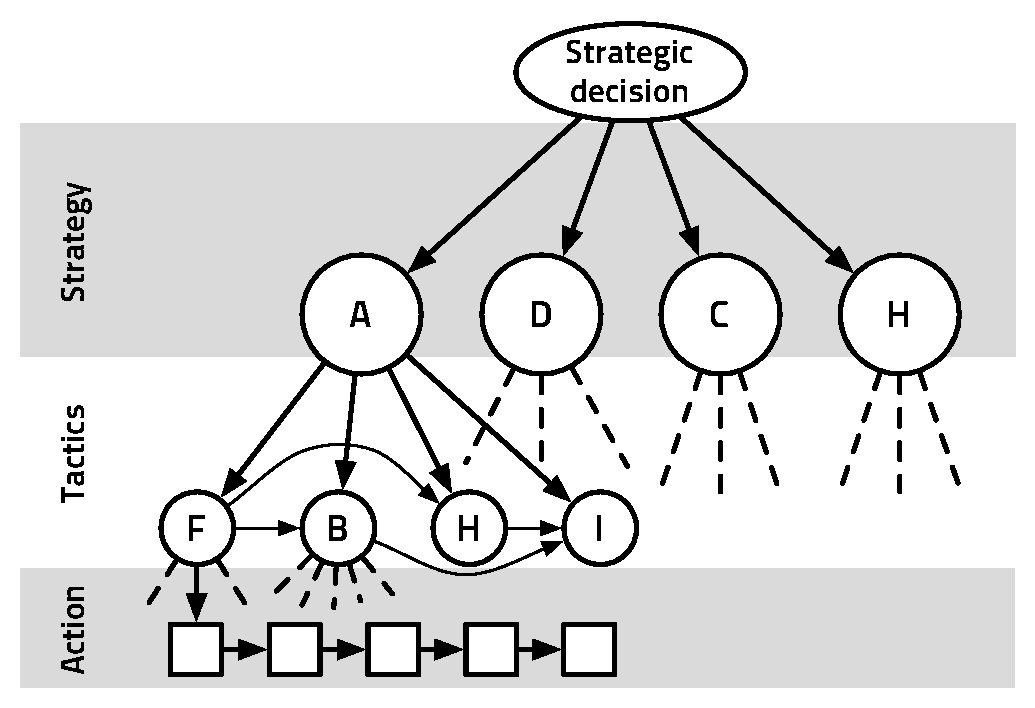
\includegraphics[width=10cm]{images/basic_abstract_decision_hierarchy3.pdf}
\end{center}
\caption{Abstract decision hierarchy in a video game. It is segmented in abstraction levels: at the strategical level, a decision is taken in $Attack$, $Defend$, $Collect$ and $Hide$; at the tactical level, it is decided between $Front$, $Back$, $Hit-and-run$, $Infiltrate$; and at the actions level between the player's possible interactions with the world.}
\label{fig:abstractdecisionhierarchy}
\end{figure}

\subsubsection{Vertical continuity}
In the decision-making process, vertical continuity describes when taking a higher-level decision implies a strong conditioning on lower-levels decisions. As seen on Figure~\ref{fig:verticalcont}: higher level abstractions have a strong conditioning on lower levels. For instance, and in non-probability terms, if the choice of a strategy $s$ (in the domain of $S$) entails a strong reduction in the size of the domain of $T$, we consider that there is a vertical continuity between $S$ and $T$. There is vertical continuity between $S$ and $T$ if $\forall s \in \{S\}, \{P(T^t|[S^t=s], T^{t-1}, O_{1:n}^t) > \epsilon\}$ is sparse in $\{P(T^t|T^{t-1}, O_{1:n}^t) > \epsilon\}$. There can be local vertical continuity, for which the previous statement holds only for one (or a few) $s \in \{S\}$, which are harder to exploit. Recognizing vertical continuity allows us to explore the state space efficiently, filtering out absurd considerations with regard to the higher decision level(s).

\begin{figure}
%%%\hspace{-0.8cm}
\begin{center}
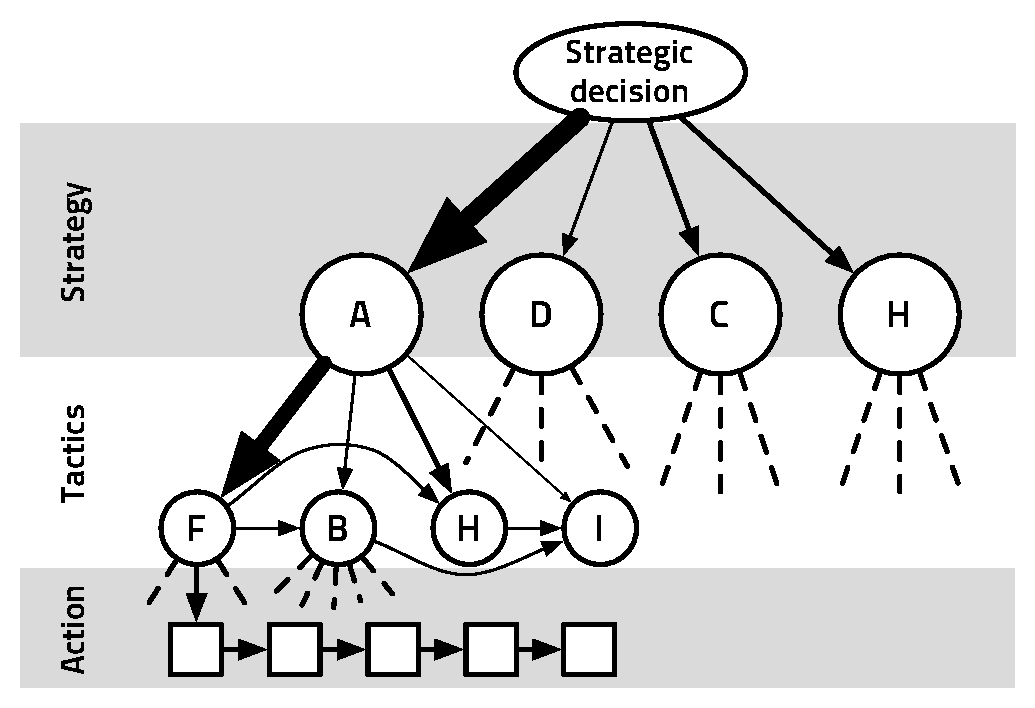
\includegraphics[width=10cm]{images/vertical_cont_abstract_decision_hierarchy3.pdf}
\end{center}
\caption{Vertical continuity in decision-making in a video game. There is a high vertical continuity between strategy and tactics as $P([T^t=Front]|[S^t=Attack], T^{t-1}, O_{1:n}^t)$ is much higher than other values for }
\label{fig:verticalcont}
\end{figure}

Examples? To edit, to choose with Pierre, ideas (+ point out example ``filtering out''):\\
navigation: S=always go north, T -> limited\\
whatever 2 player game: S=imitate, T -> limited\\
RTS: S=short term win by all-in, T -> limited\\
simpler examples?


\subsubsection{Horizontal continuity}
Horizontal continuity also helps out cutting the search in the state space to only relevant states. At a given abstraction level, it describes when taking a decision implies a strong conditioning on the next time-step decision (for this given level). As seen on Figure~\ref{fig:horizontalcont}: previous decisions on a given level have a strong conditioning on the next ones. For instance, and in non-probability terms, if the choice of a tactic $t$ (in the domain of $T^t$) entails a strong reduction in the size of the domain of $T^{t+1}$, we consider that $T$ has horizontal continuity. There is horizontal continuity between $T^{t-1}$ and $T^t$ if $\forall t in \{T\}, \{P(T^t|S^t,[T^{t-1}=t],O_{1:n}^t) > \epsilon\}$ is sparse in $\{P(T^t|S^t,O_{1:n}^t) > \epsilon\}$. There can be local horizontal continuity, for which the previous state holds only for one (or a few) $t \in \{T\}$. Recognizing horizontal continuity boils down to recognizing sequences of (frequent) actions (/?\ sequence mining ?) from decisions/actions dynamics and use that to reduce the search space of subsequent decisions. Of course, at a sufficiently small time-step, most continuous games have high horizontal continuity: the value of the time-step counts in the analysis (as the design of the abstraction levels for vertical continuity).

\begin{figure}
%%%\hspace{-0.8cm}
\begin{center}
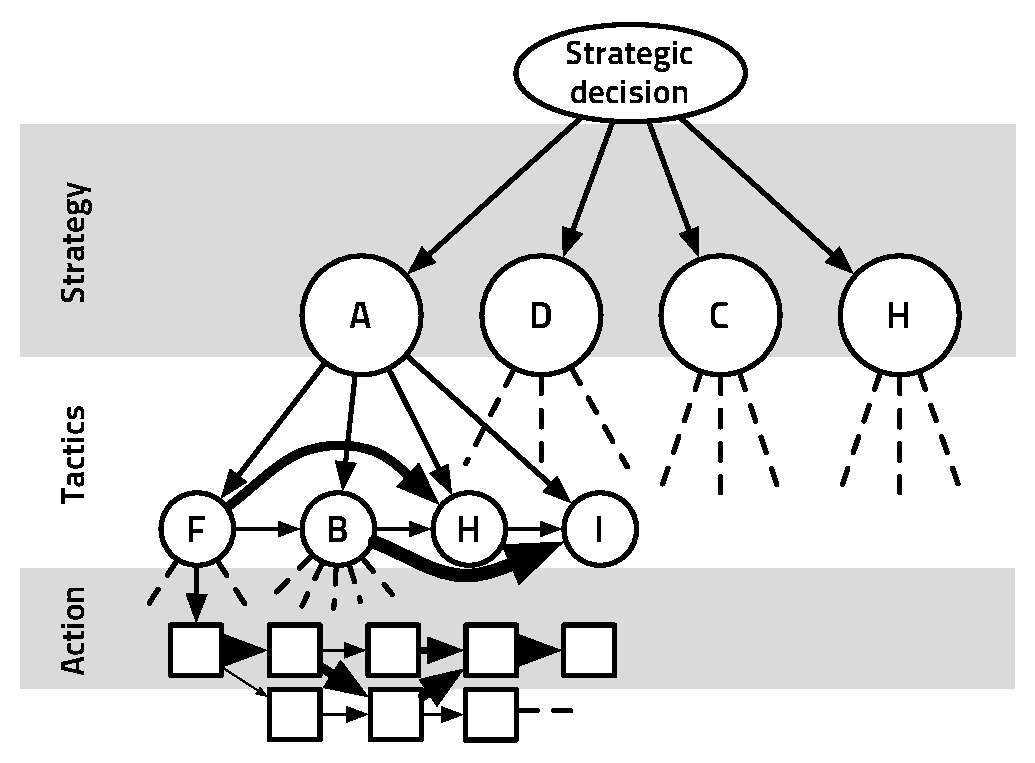
\includegraphics[width=10cm]{images/horizontal_cont_abstract_decision_hierarchy3.pdf}
\end{center}
\caption{Horizontal continuity in decision-making in a video game}
\label{fig:horizontalcont}
\end{figure}

Examples? To edit, to choose with Pierre, ideas (+ point out example ``filtering out''):\\
navigation: $T^t$=go round the block, $T^{t+1}$ -> limited by future position\\
RTS: cannot switch between Front and Back attacks with the same army at close time-steps\\
simpler examples?

\subsection{Randomness}
Randomness can be inherent to the gameplay. In board games and table top role-playing, randomness often comes from throwing dice(s) to decide the outcome of actions. In decision-making theory, this induced stochasticity is dealt with in the framework of a \newacronym{mdp}{MDP}{Markov decision process}\gls{mdp}. A \gls{mdp} is a tuple of $(S,A,T,R)$ with:
\begin{itemize}
    \item $S$ a finite set of states
    \item $A$ a finite set of actions
    \item $T_a(s,s') = P([S^{t+1}=s']|[S^t=s],[A^t=a])$ the probability that action $a$ in state $s$ at time $t$ will lead to state $s'$ at time $t+1$
    \item $R_a(s,s')$ the immediate reward for going from state $s$ to state $s'$ with action $a$.
\end{itemize}
\gls{mdp} can be solved through dynamic programming or the Bellman value iteration algorithm \citep{CitationNeeded}. In video games, the sheer size of $S$ and $A$ make it in-tractable to use \gls{mdp} directly on the whole AI task, but they are used (in research) either locally or at abstracted levels of decision. Randomness inherent to the process is one of the sources of intentional uncertainty, and we can consider player's intentions in this stochastic framework. Modeling this source of uncertainty is part of the challenge of writing game AI models.

\subsection{Partial observations}
Partial information is another source of randomness, which is found in shi-fu-mi, poker, \glos{RTS} and \glos{FPS} games, to name a few. We will not go down to the fact that the throwing of the dice seemed random because we only have partial information about its physics, or of the seed of the deterministic random generator that produced its outcome. Here, partial observations refer to the part of the game state which is deliberatively hidden between players (from a gameplay point of view): hidden hands in poker or hidden units in \glos{RTS} games due to the ``fog of war''. In decision-making theory, partial observations are dealt with in the framework of a \newacronym{pomdp}{POMDP}{partially observable Markov decision process}\gls{pomdp}. A \gls{pomdp} is a tuple $(S,A,O,T,\Omega,R)$ with $S,A,T,R$ as in a \gls{mdp} and:
\begin{itemize}
    \item $O$ a finite set of observations
    \item $\Omega$ conditional observations probabilities specifying: $P(O^{t+1}|S^{t+1},A^t)$
\end{itemize}
In a \gls{pomdp}, one cannot know exactly which state they are in and thus must reason with a probability distribution on $S$. $\Omega$ is used to update the distribution on $S$ (the belief) uppon taking the action $a$ and observing $o$, we have: $P([S^{t+1}=s']) \propto \Omega(o|s',a).\sum_{s \in S} T_a(s,s').P([S^t=s])$. In game AI, \gls{pomdp} are computationally intractable for most problems, and thus we need to model more carefully (without full $\Omega$ and $T$) the dynamics and the information value.
% \Omega([O^{t+1}=o]|[S^{t+1}=s'],[A^t=a])

%%%\subsection{Multiplayer}
%%%\subsection{PvE}

\subsection{Time Constant(s)}

\subsection{Learning Curve}

\subsection{Recap}

%%% \begin{tabular}{|l|c|c|}
%%% \hline
%%%  & Perfect information & Imperfect information \\
%%% \hline
%%% No chance & Chess & Battleship \\
%%%           & Go    & FFPS \\
%%%           &       & \textbf{RTS} \\
%%% Chance    & Monopoly & Poker \\
%%%           & \textbf{RPG} & RPG, RTS\\
%%% \hline
%%% \end{tabular}

\begin{sidewaystable}
\begin{tabular}{|l|ccccc|}
\hline 
Game & Combinatory & Vertical cont. & Horizontal cont. & Partial Info. & Randomness \\
\hline
Checkers & $b\approxeq 10; n\approxeq 70$ & none & none & no & no \\
Chess & $b\approxeq 35; n\approxeq 80$ & none & none & no & no \\
Go & $b\approxeq 250-300; n\approxeq 150-200$ & none & some & no & no \\
%Monopoly 
%Battleship
Limit Poker & $b\approxeq 3$\footnote{fold,check,raise} $;n/hour \in [20\dots240]$\footnote{number of decisions taken per hour} & some & few & much & much \\
Time Racing & $b\approxeq 50-1,000$\footnote{$\{\ddot{x} \times \theta (\times \phi)\}$ sampling$\times$50Hz}$;n/min \approxeq 60+$ & full & much & no & no \\
(TrackMania) & & & & & \\
Team FPS & $b\approxeq 100-2,000$\footnote{\label{samplingFPS}$\{X \times Y \times Z\}$ sampling$\times$50Hz + firing} $;n/min \approxeq 100$\footnote{\label{apmFPS}60 ``continuous move actions''+ 40 (mean) fire actions per sec} & some & much & some & some \\
(Counter-Strike) & & & & & \\
(Team Fortress 2) & & & & & \\
FFPS duel & $b\approxeq 200-5,000$\footref{samplingFPS} $;n/min \approxeq 100$\footref{apmFPS} & some & much & some & ($\approxeq$)no \\
(Quake III) & & & & & \\
MMORPG & $b\approxeq 50-100$\footnote{in RPGs, the player does not have to aim and positioning plays a lesser role than in FPS} $;n/min \approxeq 60$\footnote{move and use abilities/cast spells} & much & much & few & moderate \\
(WoW, DAoC) & & & & & \\
RTS & $b\approxeq 200$\footnote{atomic dir/unit $\times$ \# units + constructions + productions}$;n/min=APM\approxeq 300$\footnote{for pro-gamers, counting group actions as only one action}& some & some & much & no\\
(StarCraft) & & & & & \\
\hline
\end{tabular}
\end{sidewaystable}

%%%%%%%%%%%%%%%%%%%%%%%%%%%%%%%%%%%%%%%%%%%%%%%%%%%%%%%%%%%%%%%%%% 

\section{Player Characteristics}

%%% Timings, reflexes, modeling, goals, utility, backtracking, induction, ...

In all these games, knowledge and learning plays a key role. Humans compensate their lack of (conscious) computational power with pattern matching, abstract thinking and efficient memory structures. Between 20 and 108 answers XXX
\subsection{Virtuosity}
Skill
\subsection{Deduction}
\subsection{Induction}
\subsection{Decision-Making}
%%%\subsection{Psychology}
\subsection{Recap}
%%% https://en.wikipedia.org/wiki/Cognition
\begin{sidewaystable}
\begin{tabular}{|l|ccccccc|}
\hline 
Game & Virtuosity & Deduction & Induction & Decision-Making & \multicolumn{3}{c|}{Knowledge} \\
     & (sensory-motor) & (analysis) & (abstraction) & (acting) & game & map & opponent \\
Checkers &   & ++ & &   & ++& &+ \\
Chess &   & ++ & &   & ++& &+ \\
Go &   & ++ & + &   & ++& &+ \\
Limit Poker &   & + & + & ++ & ++& &++ \\
Time Racing & ++ &   &   &   & +&++&  \\
(TrackMania) & & & & & & & \\
Team FPS & & & & & & & \\ 
(Counter-Strike) & & & & & & & \\ 
(Team Fortress 2) & & & & & & & \\ 
FFPS duel & ++ & + &   & + & +&++&+ \\
(Quake III) & & & & & & & \\ 
MMORPG & + & + & + & ++ & +&++&+ \\
(WoW, DAoC) & & & & & & & \\ 
RTS & ++ & ++ & ++ & ++ & ++&+&++ \\
(StarCraft) & & & & & & & \\
\hline
\end{tabular}
\end{sidewaystable}

%%%%%%%%%%%%%%%%%%%%%%%%%%%%%%%%%%%%%%%%%%%%%%%%%%%%%%%%%%%%%%%%%% 

\section{An interesting problem}
\subsection{Simulated but stochastic}
Human players (ally or foes), and sometimes (most of the time) stochasticity in the rules of the game (fog of war, randomness, etc.).
